\documentclass{beamer}
\mode<presentation>
{
  \usetheme{AnnArbor}      % or try Darmstadt, Madrid, Warsaw, ...
  \usecolortheme{beaver} % or try albatross, beaver, crane, ...
  \usefonttheme{default}  % or try serif, structurebold, ...
  \setbeamertemplate{navigation symbols}{}
  \setbeamertemplate{caption}[numbered]
} 

\usepackage[english]{babel}
\usepackage[utf8x]{inputenc}
\usepackage{graphicx}
\usepackage{amsmath}
\usepackage{tikz}
\usepackage{xcolor}
\usepackage{calc}

\title[Understandin regression results]{Regression Vs. ANOVA:\\Is a main effect really a main effect?}
\author[A. Capelier-Mourguy]{Arthur Capelier-Mourguy}
\institute{Lancaster University}
\date{17th of July 2018}

\begin{document}

\begin{frame}
  \titlepage
\end{frame}

\begin{frame}{Outline}
  \tableofcontents
\end{frame}

\section{Introduction}

\subsection{Defining the problem}

\begin{frame}{Defining the problem}

  \begin{exampleblock}{What you might see}
  We defined a regression model $\texttt{Score} \sim \texttt{\alt<1>{Condition*PrePost}{Condition + PrePost + Condition:PrePost}}$.\pause
  
  \pause
  We found a significant main effect of Condition, with higher scores in the group A than in the group B.
  
  \pause
  $[$Table with parameter estimates and statistics$]$
  \end{exampleblock}
  \vspace{1em}
  \pause
  \begin{itemize}
    \item What does the regression model actually do?
    \item What do the parameter values in the table mean?
    \item What does ``main effect'' mean in the context of a regression?
  \end{itemize}
  \vspace{1em}
  \pause
  \centering{\emph{All stats in R have the same syntax}}

\end{frame}

\subsection{Content of this talk}

\begin{frame}{What to expect from this talk?}

  \vfill
  \begin{block}{What this talk is about}
    \begin{itemize}
      \item Demonstrate how ANOVA and regression results differ
      \item Detail what parameters in a regression model mean and do
    \end{itemize}
  \end{block}
  \vfill
  \pause
  \begin{block}{What this talk is not about}
    \begin{itemize}
      \item How to use R
      \item How to build a good mixed-effects model
      \item The $p$-value debate
    \end{itemize}
  \end{block}
  \vfill

\end{frame}

\section{Toy Example}

\subsection{Using categorical variables only}

\begin{frame}{The simulated data with two categorical variables}
  
  \vfill
  Assessing stress levels after and before a 30 minutes intervention, ``mindfulness meditation'' or ``video games''.
  \vfill
  \pause
  \begin{center}
  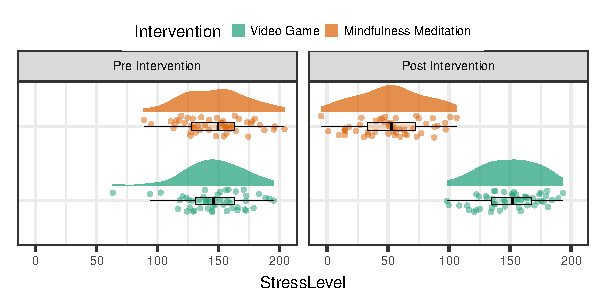
\includegraphics{../src/CategoricalRaincloud.pdf}
  \end{center}
  \vfill
  \scriptsize{``Raincloud'' plot: \url{https://micahallen.org/2018/03/15/introducing-raincloud-plots/}}

\end{frame}

\begin{frame}[fragile]{ANOVA and regression results}

	\pause
	\begin{block}{ANOVA results}
		\verb|aov(StressLevel ~ Intervention*PrePost)|
		\begin{tabular}{lccc}
		Parameter            & Sum Square & F value & $Pr(>\mathrm{F})$   \\
		\hline
		Intervention         &     114381 &   164.8 & $<2\mathrm{e}{-16}$ \\
		PrePost              &     185059 &   266.7 & $<2\mathrm{e}{-16}$ \\
		Intervention:PrePost &     102808 &   148.2 & $<2\mathrm{e}{-16}$ \\
		\end{tabular}
	\end{block}
	
	\pause
	\begin{block}{Regression results}
		\verb|lm(StressLevel ~ Intervention*PrePost)|
		\begin{tabular}{lcccc}
		Parameter                             & Estimate & Std. Error & $t$ value & $Pr(>|t|)$          \\
		\hline
		(Intercept)                           &  147.305 &      3.674 &    40.099 & $<2\mathrm{e}{-16}$ \\
		Intervention\uncover<4>{Meditation}   &    1.801 &      5.195 &     0.347 & 0.729               \\
		PrePost\uncover<4>{Post Intervention} &    3.553 &      5.195 &     0.684 & 0.495               \\
		Intervention:PrePost                  & -104.193 &      7.347 &   -14.182 & $<2\mathrm{e}{-16}$ \\
		\end{tabular}
	\end{block}

\end{frame}

\begin{frame}{Graphically understanding the regression results}

	\[Stress = 147.5 + 2 \times Int + 3.5 \times PrPo - 104 \times Int \times PrPo\]
	\[Int =
	\left\{
		\begin{array}{l}
			0\ \text{if Video Game}\\
			1\ \text{if Meditation}
		\end{array}
	\right.\mkern-9mu,\
	PrPo =
	\left\{
		\begin{array}{l}
			0\ \text{if Pre Intervention}\\
			1\ \text{if Post Intervention}
		\end{array}
	\right.\]
	
	\begin{overlayarea}{\textwidth}{2.5in}
	\only<2-3>{For Video Game Pre Int.,
		\alt<3>{\(Stress = 147.5\)}{\(Stress = 147.5 + 2 \times 0 + 3.5 \times 0 - 104 \times 0 \times 0\)}
	}
	\only<4-5>{For Meditation Pre Int.,
		\alt<5>{\(Stress = 147.5 + 2\)}{\(Stress = 147.5 + 2 \times 1 + 3.5 \times 0 - 104 \times 1 \times 0\)}
	}
	\only<6-7>{For Video Game Post Int.,
		\alt<7>{\(Stress = 147.5 + 3.5\)}{\(Stress = 147.5 + 2 \times 0 + 3.5 \times 1 - 104 \times 0 \times 1\)}
	}
	\only<8->{For Meditation Post Int.,
		\alt<9->{\(Stress = 147.5 + 2 + 3.5 - 104\)}{\(Stress = 147.5 + 2 \times 1 + 3.5 \times 1 - 104 \times 1 \times 1\)}
	}
	
	\begin{center}
		\invisible<1>{
			\definecolor{VG}{RGB}{27,158,119}
			\definecolor{MM}{RGB}{217,95,2}
			\definecolor{param0}{RGB}{117,112,179}
			\definecolor{param1}{RGB}{231,41,138}
			\definecolor{param2}{RGB}{102,166,30}
			\definecolor{param3}{RGB}{230,171,2}
			\begin{tikzpicture}[scale = .26]
				\tikzstyle{every node}=[font=\footnotesize]
				% Grid
				\draw (4,17) -- (4, 1) -- (20,1);
				% y axis
				\node[rotate = 90] at (0, 10){Stress Level};
				\draw (3.5, 16) -- (4, 16); \node at (2.25, 16){150};
				\draw (3.5, 11) -- (4, 11); \node at (2.25, 11){100};
				\draw (3.5, 6) -- (4, 6); \node at (2.25, 6){50};
				\draw (3.5, 1) -- (4, 1); \node at (2.25, 1){0};
				% x axis
				\draw (8, 0.7) -- (8, 1); \node at (8, 0){Pre Int.};
				\draw (16, 0.7) -- (16, 1); \node at (16, 0){Post Int.};
				% Intercept
				\only<3>{\draw[thick, color=param0, <->] (8, 1) -- (8, 15.75) node[pos=.5, right]{Intercept};}
				\only<3->{\filldraw[VG] (7.5, 15.75) circle (.25);}
				% Intervention
				\only<5>{\draw[thick, color=param1, -] (8, 15.75) -- (8, 15.95) node[below]{Intervention};}
				\only<5->{\filldraw[MM] (8.5, 15.95) circle (.25);}
				% PrePost
				\only<7>{
					\draw[dashed, gray] (7.75, 15.75) -- (16.25, 15.75);
					\draw[thick, color=param2, -] (16, 15.75) -- (16, 16.1) node[pos=.5, right]{PrePost};
				}
				\only<7->{\filldraw[VG] (15.5, 16.1) circle (.25);}
				% Interaction
				\only<9->{
					\draw[dashed, gray] (7.75, 15.75) -- (16.25, 15.75);
					\draw[thick, color=param2, -] (16.25, 15.75) -- (16.25, 16.1) node[below right]{PrePost};
				}
				\uncover<10->{\draw[thick, color=param1, -] (16.25, 16.1) -- (16.25, 16.3) node[right]{Intervention};}
				\only<11->{\draw[thick, color=param3, <->] (16, 16.3) -- (16, 5.9) node[pos=.5, right]{Interaction};}
				\only<11->{\filldraw[MM] (16.5, 5.9) circle (.25);}
			\end{tikzpicture}
		}
	\end{center}
	\end{overlayarea}

\end{frame}

\begin{frame}{Impact of the choice of reference levels}

	\pause
	Let's redefine Intervention: 0 = Meditation, 1 = Video Game.
	\pause
	\vspace{.5em}

	\begin{tabular}{lcccc}
		Parameter                & Estimate & Std. Error & $t$ value & $Pr(>|t|)$          \\
		\hline
		(Intercept)              &  149.106 &      3.674 &    40.589 & $<2\mathrm{e}{-16}$ \\
		InterventionVideo Game   &   -1.801 &      5.195 &    -0.347 & 0.729               \\
		PrePostPost Intervention & -100.640 &      5.195 &   -19.372 & $<2\mathrm{e}{-16}$ \\
		Intervention:PrePost     &  104.193 &      7.347 &    14.182 & $<2\mathrm{e}{-16}$ \\
	\end{tabular}
	\pause
	
	\begin{center}
		\definecolor{VG}{RGB}{27,158,119}
		\definecolor{MM}{RGB}{217,95,2}
		\definecolor{param0}{RGB}{117,112,179}
		\definecolor{param1}{RGB}{231,41,138}
		\definecolor{param2}{RGB}{102,166,30}
		\definecolor{param3}{RGB}{230,171,2}
		\begin{tikzpicture}[scale = .25]
			\tikzstyle{every node}=[font=\footnotesize]
			% Grid
			\draw (4,17) -- (4, 1) -- (20,1);
			% y axis
			\node[rotate = 90] at (0, 10){Stress Level};
			\draw (3.5, 16) -- (4, 16); \node at (2.25, 16){150};
			\draw (3.5, 11) -- (4, 11); \node at (2.25, 11){100};
			\draw (3.5, 6) -- (4, 6); \node at (2.25, 6){50};
			\draw (3.5, 1) -- (4, 1); \node at (2.25, 1){0};
			% x axis
			\draw (8, 0.7) -- (8, 1); \node at (8, 0){Pre Int.};
			\draw (16, 0.7) -- (16, 1); \node at (16, 0){Post Int.};
			% Intercept
			\only<5->{\draw[thick, color=param0, <->] (7.8, 1) -- (7.8, 15.9) node[pos=.5, right]{Intercept};}
			\filldraw[MM] (7.5, 15.9) circle (.25);
			% Intervention
			\only<6->{\draw[thick, color=param1, -] (8.2, 15.9) -- (8.2, 15.7) node[below right]{Intervention};}
			\filldraw[VG] (8.5, 15.7) circle (.25);
			% PrePost
			\only<7->{
				\draw[dashed, gray] (7.75, 15.9) -- (16.25, 15.9);
				\draw[thick, color=param2, <->] (15.8, 15.9) -- (15.8, 4.85) node[pos=.5, left]{PrePost};
			}
			\filldraw[MM] (15.5, 4.85) circle (.25);
			% Interaction
			\uncover<8>{\draw[thick, color=param1, -] (16.2, 4.85) -- (16.2, 5.05) node[right]{Intervention};}
			\only<8>{\draw[thick, color=param3, <->] (16.2, 5.05) -- (16.2, 15.55) node[pos=.5, right]{Interaction};}
			\filldraw[VG] (16.5, 15.55) circle (.25);
		\end{tikzpicture}
	\end{center}

\end{frame}

\subsection{Using continuous variables}

\begin{frame}{A slightly less meaningfull example with a continuous variable}

	\vfill
	Assessing the difference between treatment A and treatment B in reducing stress levels each day over a week.
	\pause
	\vfill
	
	\begin{center}
		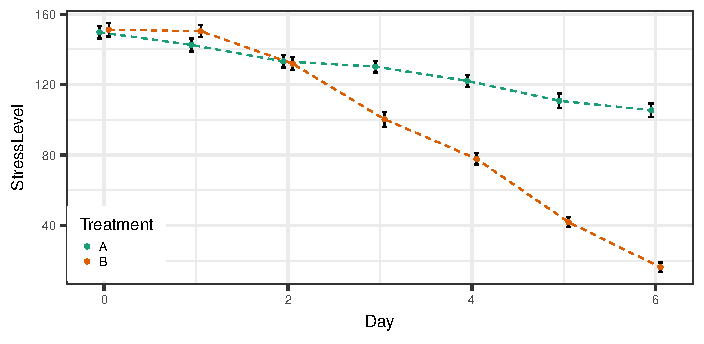
\includegraphics{../src/Continuous.pdf}
	\end{center}
	\vfill

\end{frame}

\begin{frame}{Regression results}

	\begin{center}
		\begin{tabular}{lcccc}
		Parameter      & Estimate & Std. Error & $t$ value & $Pr(>|t|)$           \\
		\hline
		(Intercept)    & 149.9317 &     2.5003 &    59.967 & $<2\mathrm{e}{-16}$  \\
		TreatmentB     &  18.1489 &     3.5359 &     5.133 & $3.71\mathrm{e}{-7}$ \\
		Day            &  -7.4051 &     0.6934 &   -10.679 & $<2\mathrm{e}{-16}$  \\
		TreatmentB:Day & -16.7244 &     0.9807 &   -17.054 & $<2\mathrm{e}{-16}$  \\
		\end{tabular}
		
		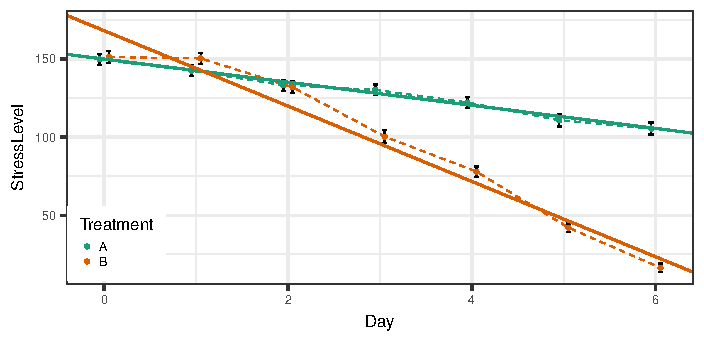
\includegraphics[height=2.07in]{../src/ContinuousPred.pdf}
	\end{center}

\end{frame}

\section{Real Data Example}

\subsection{Methods}

\begin{frame}{The experiment in a nutshell}

  Categorisation and labelling in 15-month-old infants.
  \vspace{2em}
  \begin{description}
    \pause\item[\hspace{37.5pt}Conditions] Label and no-label.
    \pause\item[\hspace{20pt}Familiarisation] Snake-like animal with a head and a tail.
    
    Label condition: categories defined by the tail.
    \pause\item[Novelty Preference] Did they encode the tail? The head?
    
    One old animal against one animal with a new head/tail.
  \end{description}

\end{frame}

\subsection{Results}

\begin{frame}{Choosing reference levels}

  \begin{center}
    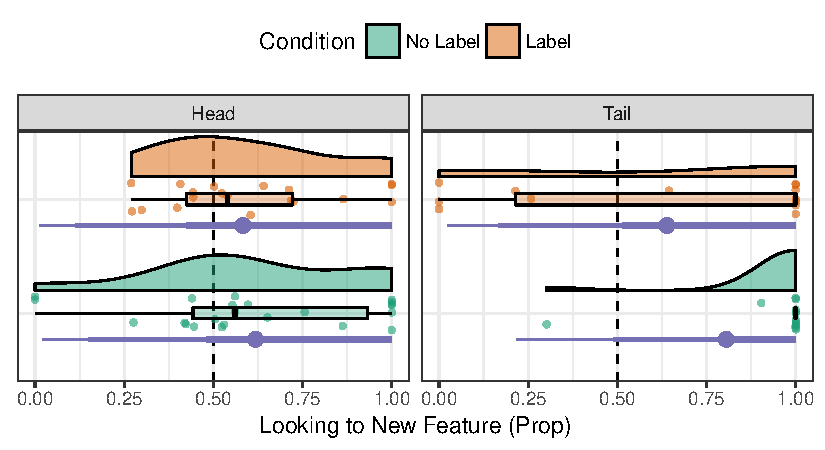
\includegraphics[height=2.5in]{SalDi-old_new.pdf}
  \end{center}

\end{frame}

\section{Conclusion}

\begin{frame}{What's the take home message?}

  \begin{itemize}
    \pause\item Don't assume you know what your model's parameters mean
    \pause\item Break down the model formula case-by-case
    \pause\item Plot model predictions
    \pause\item Ask online\pause: StackOverflow\pause, Cross Validated\pause, Github\pause, Twitter
  \end{itemize}
  \vspace{3em}
  \pause
  \centering{\emph{Thanks for listening!}}

\end{frame}

\end{document}
